\documentclass[
a4paper,   
headsepline, 
fleqn,     
12pt
]{scrartcl}

%%% ngerman: language set to new-german
\usepackage{ngerman}
\usepackage[latin1]{inputenc}
\usepackage[T1]{fontenc}
\usepackage{ae,aecompl}

%%% Graphic stuff
\usepackage{graphicx}
\usepackage{amsmath,amssymb,amstext}
\usepackage{units}
\usepackage{scrpage2}

%%% comments, ...
\usepackage{verbatim}

\setlength{\parindent}{0em} 

\newcommand{\mygraphics}[3]{
  \begin{center}
    \includegraphics[width=#1, keepaspectratio=true]{#2} \\
    \textbf{#3}
  \end{center}
}

%%%      footer - middle: page number
\pagestyle{scrheadings}

%%% heading - left
 \ihead[]{Marco Sohm, Kevin Wallis}

%%% heading - right
 \ohead[]{Aufgabe 2}

\begin{document}

 \pagenumbering{roman} %% small roman page numbers
 \pagenumbering{arabic} 

\subsection*{Einleitende Worte}
Die offene Arbeit wird in Stunden angegeben. Arbeitet ein Mitarbeit zu $100$\% am Projekt, dann schafft er es acht (Leistungsumrechnungfaktor) Stunden pro Tag abzuarbeiten.
Da ein Mitarbeiter aber nie zu $100$\% am Projekt arbeiten kann, gibt es die Leistungsfaktoren. Alle im Model verwendeten Funktionen sind in Prozent angegeben und mit dem Leistungsumrechnungfaktor verbunden. So bedeutet $Integrationsverluste\_MIE(MitarbeiterInEinarbeitung)$ f�r $Argument = 2$ und $Value = 12,5$, dass bei zwei Mitarbeitern in Einarbeitung eine Stunde (= 0,125 * 8) pro Tag f�r die Integration eingeplant werden muss.
\\ \\
Annahme: Die Teamdynamik kann den Interaktionsverlust maximal um den Faktor zwei halbieren.
Interaktion findet auch bei MitarbeiterInEinarbeitung statt. Diese wird jedoch in den Integrationsverlust einbezogen. Wochenenden und Ferien werden nicht modelliert.

\subsection*{zu a) Ideen hinter der Modellierung}
\begin{comment}
a) Versuchen Sie, das Modell soweit zu bringen, da� plausible Simulationsresultate zu beobachten sind. Falls Sie dazu selbst�ndig Information in das Modell hineingebracht haben, die nicht im Buchkapitel angegeben wurden, begr�nden Sie Ihre Wahl mit vollst�ndigen S�tzen. Suchen Sie auch danach, wo sinnvollerweise realistische Reaktionszeiten einzubauen sind. Bauen Sie sie dann ein und beobachten Sie das Resultat.
\end{comment}
Startwerte k�nnen dem AnyLogic-Model entnommen werden. \\
Einzelne Funktionen k�nnten beschrieben werden: z.B. \\
$Interaktionsverlust = InteraktionsverlustFunktion(VerfuegbareMitarbeiter)  - Teamdynamik$
wobei 
$Teamdynamik = VerfuegbareMitarbeiter/ Integration$
Mit Erkl�rung: Warum haben wir und entschieden es so zu modellieren?
Die Teamdynamik ist abh�ngig von den Verf�gbarenMitarbeitern, je mehr Mitarbeiter desto besser die Teamdynamik (wobei es auch irgendwie ein Maximum geben sollte -> Funktion verwenden). Au�erdem je l�nger die gleichen Mitarbeiter an einem Projekt arbeiten (d.h. je kleiner die Integration), desto gr��er die Teamdynamik. Deswegen dividiert durch Integration.


\subsection*{zu b) Variation der Integration und Teamdynamik}
\begin{comment}
b) Variieren Sie Integrationszeit (also die entsprechende Rate),und die Wirkung der Teamdynamik in einem sinnvollen Bereich, und beschreiben Sie verbal und mit einem Graphen/Plot die beobachteten Ver�nderungen im System. Geben Sie einen Erkl�rungsversuch.
\end{comment}

\newpage

\subsection*{Anhang}
Die folgenden Diagramme stellen Vergleiche zu 'Der Termin' her. Dabei ist
darauf zu achten, dass Abweichungen zu den dort dargestellten Modellen bestehen. So wurde teilweise vereinfacht und/oder weitere Konzepte hinzugef�gt.

\begin{figure}[h]
  \centering
  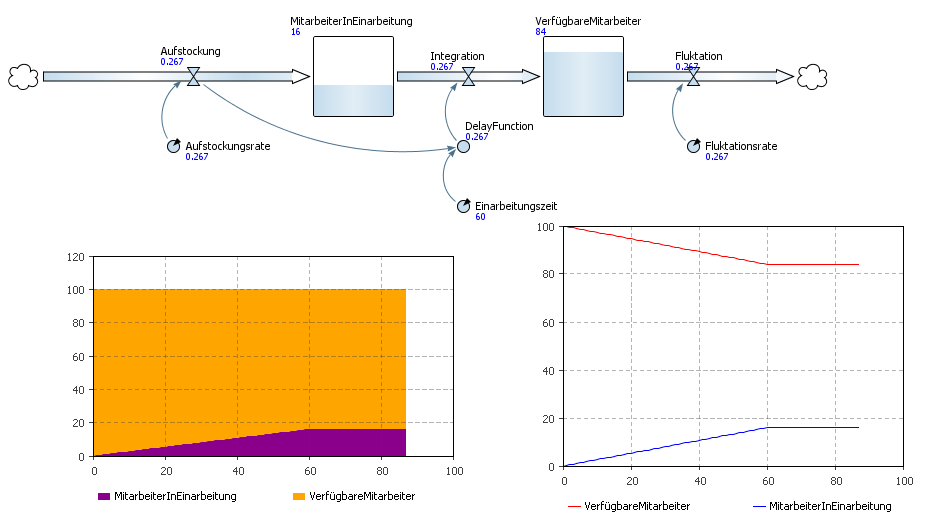
\includegraphics[width=1\textwidth]{./images/Model1_Seite8}
  \caption{Model Stage 1 (vergleiche Seite 8 'Der Termin')}
  \label{fig:Model_Seite_8}
\end{figure}

\begin{figure}[h]
  \centering
  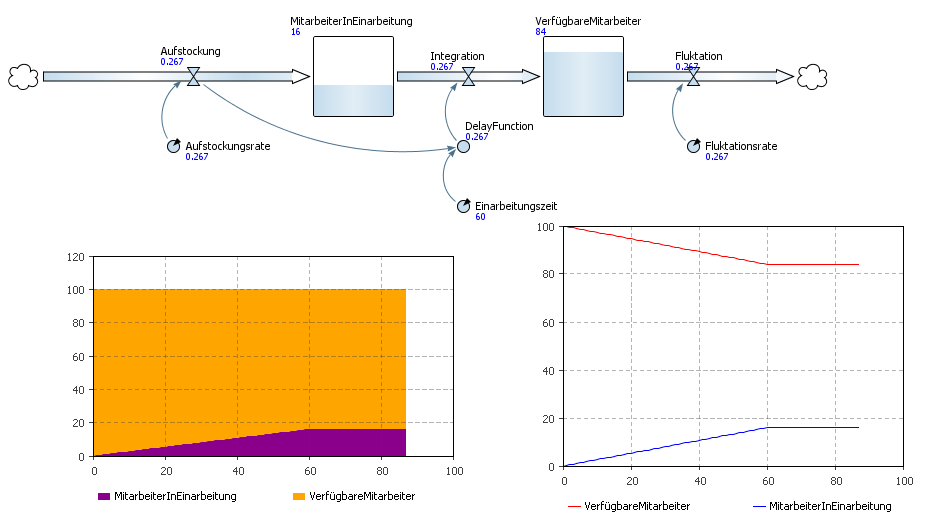
\includegraphics[width=1\textwidth]{./images/Model1_Seite14}
  \caption{Model Stage 2 (vergleiche Seite 14 'Der Termin')}
  \label{fig:Model_Seite_14}
\end{figure}

\begin{figure}[h]
  \centering
  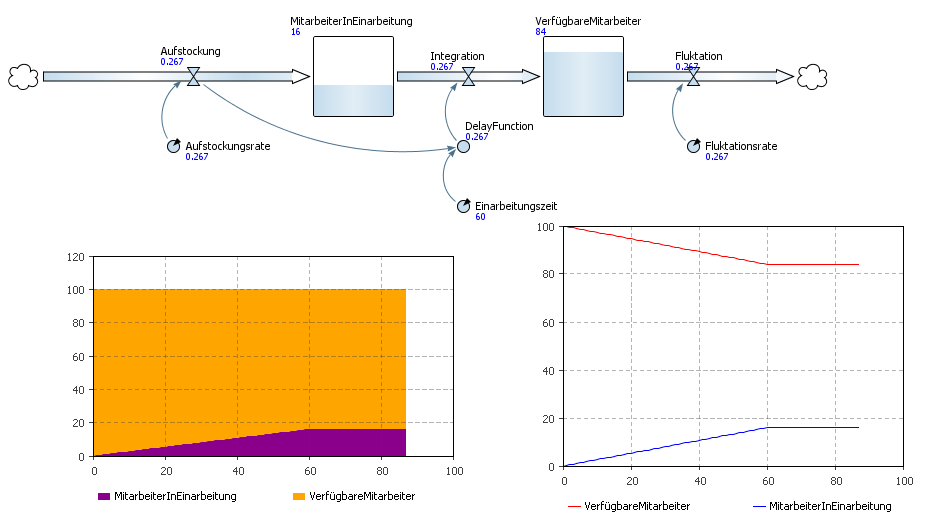
\includegraphics[width=1\textwidth]{./images/Model1_Seite16}
  \caption{Model Stage 3 (vergleiche Seite 16 'Der Termin')}
  \label{fig:Model_Seite_16}
\end{figure}

\appendix  
\bibliographystyle{plain}
\bibliography{projekt.bib}

\end{document}